\documentclass[14pt, a4paper]{article}
\usepackage[T2A]{fontenc}
\usepackage[utf8]{inputenc}
\usepackage[russian]{babel}
\usepackage[left=3cm, right=1.5cm, top=2cm, bottom=2cm]{geometry}
\usepackage{indentfirst}
\usepackage{microtype}
\usepackage{array}
\usepackage{xcolor}
% \usepackage{times}
\usepackage{tempora}
\usepackage{ulem}
\usepackage{setspace}
\usepackage{amsmath}
\usepackage{booktabs}
\usepackage{graphicx}
\usepackage{float}
\usepackage{listings}
\graphicspath{{reports/figures/}{figures/}}
\lstset{basicstyle=\ttfamily\small, breaklines=true, columns=fullflexible, frame=single, keepspaces=true}
\pagestyle{empty}

\makeatletter
\renewcommand\section{\@startsection {section}{1}{\parindent}%
  {-3.5ex \@plus -1ex \@minus -.2ex}%
  {0.5ex}%
  {\normalfont\Large\bfseries}}
\renewcommand\tableofcontents{%
  \begin{center}\Large\bfseries\contentsname\end{center}%
  \@starttoc{toc}%
}
\renewcommand*\l@section{\@dottedtocline{1}{0em}{1.5em}}
\makeatother

\begin{document}
\onehalfspacing

\begin{center}
    \textbf{ФЕДЕРАЛЬНОЕ ГОСУДАРСТВЕННОЕ АВТОНОМНОЕ ОБРАЗОВАТЕЛЬНОЕ} \\
    \textbf{УЧРЕЖДЕНИЕ ВЫСШЕГО ОБРАЗОВАНИЯ} \\
    \textbf{«МОСКОВСКИЙ АВИАЦИОННЫЙ ИНСТИТУТ} \\
    \textbf{(НАЦИОНАЛЬНЫЙ ИССЛЕДОВАТЕЛЬСКИЙ УНИВЕРСИТЕТ)»}
\end{center}

\begin{center}
    \bfseries Институт №8 «Компьютерные науки и \\
    \bfseries прикладная математика» \\
    \bfseries Кафедра 806 «Вычислительная математика \\
    \bfseries и программирование»
\end{center}

\vspace{3cm}

\begin{center}
    \Large\bfseries Отчет \\
    \vspace{0.5cm}
    \mdseries по лабораторной работе №3.5
\end{center}

\vfill

\noindent
\hfill
\begin{tabular}{ll}
Группа:       & М8О-307Б-21 \\
Студент:      & М. С. Ивченко \\
Преподаватель:& доц. В. В. Киндинова \\
Оценка:       & \underline{\makebox[3cm][c]{}} \\ [0.2cm]
Дата:         & \underline{\makebox[3cm][c]{}}
\end{tabular}

\vfill

\begin{center}
    Москва \\
    2026
\end{center}

\newpage

\setcounter{tocdepth}{2}
\tableofcontents
\newpage

\section*{Тема}
\addcontentsline{toc}{section}{Тема}
Цель данной лабораторной работы -- изучить базовые квадратурные формулы для приближенного вычисления определенных интегралов. В работе сравниваются методы прямоугольников, трапеций и Симпсона, а точность результата уточняется с помощью оценки Рунге-Ромберга.

\section*{Задание}
\addcontentsline{toc}{section}{Задание}
Вычислить определенный интеграл $F = \int_{X_0}^{X_k} y \, dx$, методами прямоугольников, трапеций, Симпсона с шагами $h_1$, $h_2$. Оценить погрешность вычислений, используя метод Рунге-Ромберга.

\section*{Теория}
\addcontentsline{toc}{section}{Теория}
Численное интегрирование заменяет определенный интеграл конечной суммой значений функции. На равномерной сетке $x_i=a+ih$, $i=0,\ldots,n$, составные квадратурные формулы применяются к каждому малому отрезку и затем суммируются.

Метод средних прямоугольников аппроксимирует функцию на каждом отрезке значением в середине:
\[
I_h=h\sum_{i=0}^{n-1}f\left(\frac{x_i+x_{i+1}}2\right),
\]
и имеет второй порядок точности. Метод трапеций использует линейную аппроксимацию на каждом отрезке:
\[
    I_h=h\left(\frac{f(x_0)+f(x_n)}2+\sum_{i=1}^{n-1}f(x_i)\right).
\]
Он также имеет второй порядок точности для достаточно гладкой функции.

Формула Симпсона применяет квадратичную интерполяцию на парах отрезков, поэтому требует четного числа промежутков:
\[
    I_h=\frac{h}{3}\left(f(x_0)+f(x_n)
    +4\sum_{\substack{i=1\\ i\ \mathrm{odd}}}^{n-1}f(x_i)
    +2\sum_{\substack{i=2\\ i\ \mathrm{even}}}^{n-2}f(x_i)\right).
\]
Ее порядок точности равен четырем.

Если значение интеграла вычислено с шагами $h$ и $h/r$, можно оценить ошибку методом Рунге--Ромберга:
\[
    R=\frac{I_{h/r}-I_h}{r^p-1}.
\]
Здесь $p$ -- порядок метода: $p=2$ для прямоугольников и трапеций, $p=4$ для Симпсона. Уточненное значение равно $I_{h/r}+R$. Такая оценка показывает, насколько результат меняется при измельчении сетки.

\begin{lstlisting}[language=Python]
correction = (fine_value - coarse_value) / ((coarse_step / fine_step) ** order - 1)
corrected = fine_value + correction
\end{lstlisting}

\section*{Ход лабораторной работы}
\addcontentsline{toc}{section}{Ход лабораторной работы}
Вычислялся интеграл
\[
    \int_{-2}^{2}\frac{dx}{x^3+64}
\]
при шагах $h_1=1.0$ и $h_2=0.5$.
\begin{table}[H]
\centering
\begin{tabular}{lrrrr}
\toprule
Метод & $I(h_1)$ & $I(h_2)$ & $|R_{RR}|$ & Уточнение\\
\midrule
Прямоугольники & 0.0625872651 & 0.0626255883 & 0.0000127744 & 0.0626383627\\
Трапеции & 0.0627556471 & 0.0626714561 & 0.0000280637 & 0.0626433925\\
Симпсон & 0.0626755189 & 0.0626433925 & 0.0000021418 & 0.0626412507\\
\bottomrule
\end{tabular}
\caption{Результаты численного интегрирования и поправка Рунге--Ромберга.}
\end{table}

\begin{figure}[H]
    \centering
    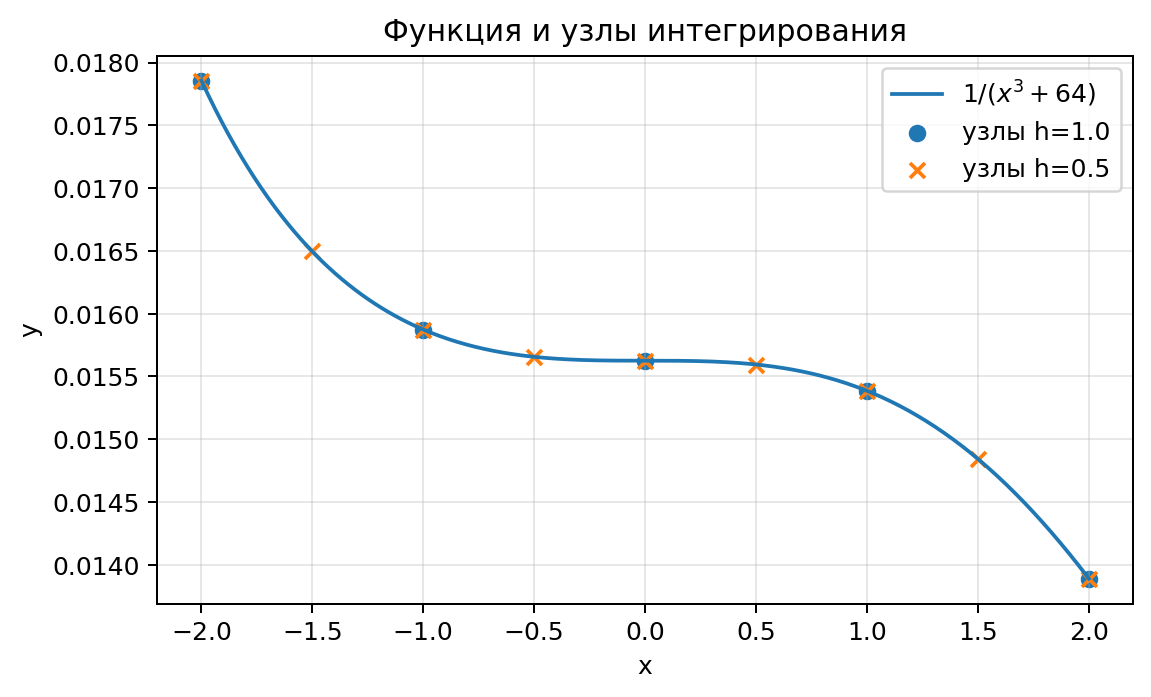
\includegraphics[width=0.86\textwidth]{lab3_5_integration.png}
    \caption{Подынтегральная функция и узлы сеток с шагами $1.0$ и $0.5$.}
\end{figure}

\section*{Выводы}
\addcontentsline{toc}{section}{Выводы}
При уменьшении шага все методы дают близкие значения интеграла. Наименьшая оценка поправки получилась у метода Симпсона, что соответствует его четвертому порядку точности.

\end{document}
